\documentclass[11pt]{article}
\usepackage[margin=0.8in]{geometry}
\usepackage[T1]{fontenc}
\usepackage{lmodern,tikz,hyperref}
\setlength{\parindent}{0pt}\setlength{\parskip}{8pt}\sloppy
\begin{document}
\begin{center}{\Large Saved retained-row accounting reconciliation}\\1 November 2026\end{center}
A native Rust read-only checker reconciled the archived input index, output dispositions and repeated setup metadata. The saved producer was not executed. No curve operations, new target trajectories, scientific measurements or cloud operations occurred.

\textbf{Historical saved-file counts.} The archive contains 180 physical rows: 60 selected by the saved index and 120 explicitly unselected. All 420 indexed case dispositions are present exactly once. The 202 compared cases contain 174 first observations and 28 redundant observations. These counts describe stored fixtures, not natural relation yields.

\begin{center}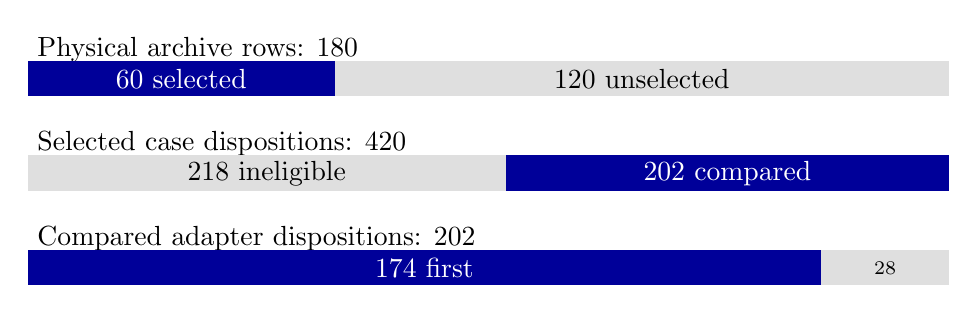
\begin{tikzpicture}[x=0.013cm,y=1cm]
\node[anchor=west] at (0,3.6) {Physical archive rows: 180};
\fill[blue!60!black] (0,3) rectangle (300,3.45);\fill[gray!25] (300,3) rectangle (900,3.45);
\node[white] at (150,3.22) {60 selected};\node at (600,3.22) {120 unselected};
\node[anchor=west] at (0,2.4) {Selected case dispositions: 420};
\fill[gray!25] (0,1.8) rectangle (467.14,2.25);\fill[blue!60!black] (467.14,1.8) rectangle (900,2.25);
\node at (233.57,2.02) {218 ineligible};\node[white] at (683.57,2.02) {202 compared};
\node[anchor=west] at (0,1.2) {Compared adapter dispositions: 202};
\fill[blue!60!black] (0,0.6) rectangle (775.25,1.05);\fill[gray!25] (775.25,0.6) rectangle (900,1.05);
\node[white] at (387.62,0.82) {174 first};\node[font=\scriptsize] at (837.62,0.82) {28};
\end{tikzpicture}\end{center}
The bars use separate denominators. The editable diagram is \texttt{ledger.svg}; standardized records and exact source hashes are in \texttt{reconciliation.json}.

\textbf{Accounting identity.} Setup and constructor metadata repeat across cases but are nonadditive copies. Each selected physical row contributes exactly once, keyed by archive SHA256 and physical row index. All repeated copies agree, and the once-per-row totals exactly match the historical saved analysis. Every archive row and observed disposition remains represented; missing counters remain null.

\textbf{Scope.} The full obligation remains 1,260 targets. Complete cost ratio and natural yield remain null. Allocation, hashing, comparisons, memory, complete primality and square-root work, process setup and matched controls are not supplied by these counters.
\newpage
\section*{Negative controls and provenance}
Four independently altered copies of saved inputs were processed. All returned native exit 1, \texttt{reconciliation\_pass=false}, and explicit discrepancy records:
\begin{itemize}
\item Duplicate a saved disposition: duplicate identity detected.
\item Remove a saved disposition: expected identity missing.
\item Alter one repeated setup counter: inconsistent per-row setup copies detected.
\item Change a workload identity: archive identity mismatch detected.
\end{itemize}
Original inputs were preserved. Controls only alter copied JSON records; they do not simulate a collection process. Individual receipts, altered-input hashes and outputs are retained under \texttt{controls/}; \texttt{controls/summary.json} records all four outcomes.

\textbf{Implementation basis.} Repository \texttt{AGENTS.md} requires native research/accounting implementation. The historical \texttt{retained-duplicate-executed/run.py} combines producer execution with analysis; its entrypoint was not run. The new Rust reader preserves the existing analysis contract and adds the archive-hash namespace, archived-case joins and explicit unselected partitions.

Input lineage:
\begin{itemize}
\item \texttt{archive.jsonl}: physical input rows and retained case witnesses.
\item \texttt{input-index.jsonl}: selected expected disposition identities.
\item \texttt{run.stdout}: historical native output records.
\item \texttt{analysis.json}: historical once-per-row totals used for comparison.
\item \texttt{receipt.json}: historical producer exit, not a new execution receipt.
\item \texttt{src/pruned.rs}, \texttt{src/duplicate.rs}, \texttt{src/graph.rs}: source boundaries for setup, disposition and graph accounting.
\end{itemize}
Exact absolute paths and SHA256 hashes are embedded in \texttt{reconciliation.json}. The final formatted Rust build and read-only run exited zero; its JSON was byte-identical to the previous successful readback. An initial compile error concerning owned JSON keys is retained as \texttt{attempt1.stderr}.

\textbf{Review boundary.} The checker reconciles saved identities and accounting metadata. It does not replay scalar certificates, prove mathematical invariants, certify timing isolation, or replace a full experiment review. Root review of the checker remains separate.
\end{document}
